\documentclass[tikz,border=2mm]{standalone}
\usepackage{fontspec,amsmath}
\IfFontExistsTF{TeX Gyre Heros}{\setmainfont{TeX Gyre Heros}}{\setmainfont{Latin Modern Sans}}
\usetikzlibrary{arrows.meta,positioning,calc}
\definecolor{ink}{HTML}{173348}
\definecolor{blue}{HTML}{246684}
\definecolor{green}{HTML}{217B70}
\definecolor{orange}{HTML}{A76523}
\tikzset{every node/.style={font=\fontsize{9}{11}\selectfont,text=ink,align=center},
box/.style={draw=blue!65,rounded corners=1mm,fill=blue!4,inner sep=2mm},
arr/.style={-{Stealth[length=1.7mm]},draw=blue,line width=.65pt}}
\begin{document}
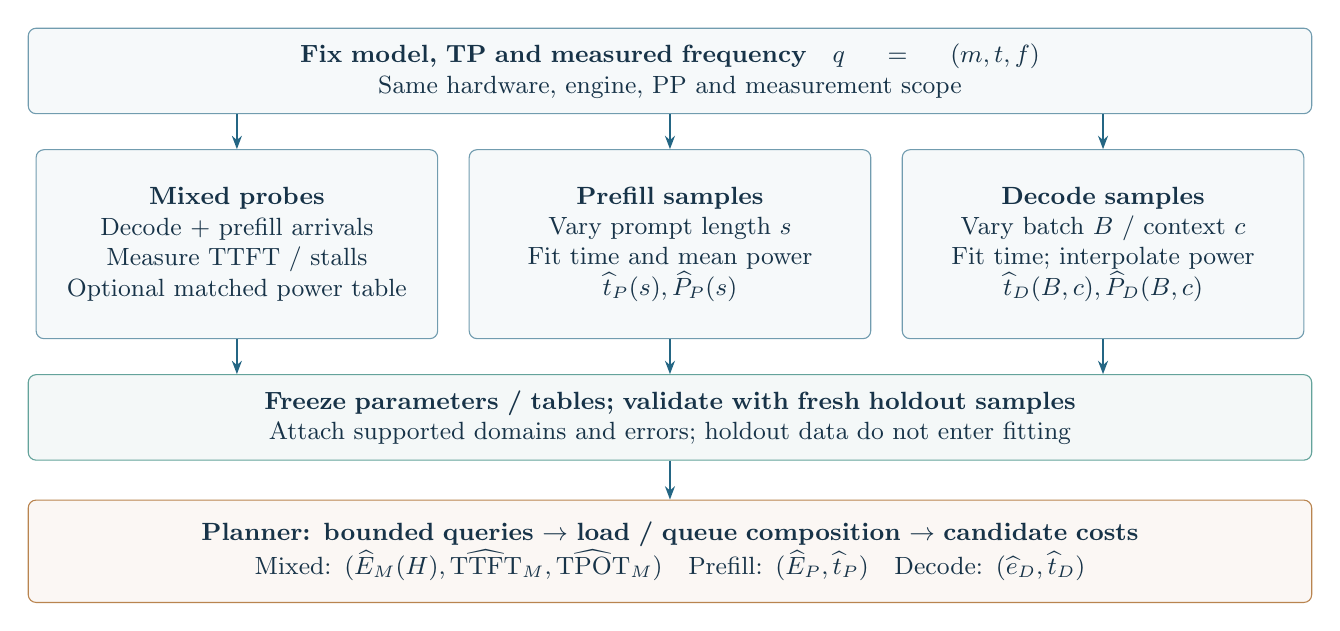
\begin{tikzpicture}[x=1mm,y=1mm]
\node[box,text width=159mm,minimum height=10mm] (q) at (80,0)
{\textbf{Fix model, TP and measured frequency}\quad $q=(m,t,f)$\\
Same hardware, engine, PP and measurement scope};
\node[box,text width=47mm,minimum height=24mm] (m) at (25,-22)
{\textbf{Mixed probes}\\Decode + prefill arrivals\\Measure TTFT / stalls\\Optional matched power table};
\node[box,text width=47mm,minimum height=24mm] (p) at (80,-22)
{\textbf{Prefill samples}\\Vary prompt length $s$\\Fit time and mean power\\$\widehat t_P(s),\widehat P_P(s)$};
\node[box,text width=47mm,minimum height=24mm] (d) at (135,-22)
{\textbf{Decode samples}\\Vary batch $B$ / context $c$\\Fit time; interpolate power\\$\widehat t_D(B,c),\widehat P_D(B,c)$};
\draw[arr] (q.south -| m.north)--(m.north);
\draw[arr] (q.south)--(p.north);
\draw[arr] (q.south -| d.north)--(d.north);
\node[box,draw=green!70,fill=green!5,text width=159mm,minimum height=10mm] (v) at (80,-44)
{\textbf{Freeze parameters / tables; validate with fresh holdout samples}\\
Attach supported domains and errors; holdout data do not enter fitting};
\draw[arr] (m.south)--(m.south|-v.north);
\draw[arr] (p.south)--(v.north);
\draw[arr] (d.south)--(d.south|-v.north);
\node[box,draw=orange!80,fill=orange!5,text width=159mm,minimum height=13mm] (o) at (80,-61)
{\textbf{Planner: bounded queries $\rightarrow$ load / queue composition $\rightarrow$ candidate costs}\\
Mixed: $(\widehat E_M(H),\widehat{\mathrm{TTFT}}_M,\widehat{\mathrm{TPOT}}_M)$\quad
Prefill: $(\widehat E_P,\widehat t_P)$\quad Decode: $(\widehat e_D,\widehat t_D)$};
\draw[arr] (v.south)--(o.north);
\end{tikzpicture}
\end{document}
